\subsection{Differentiating on the Unit Sphere}

Geometrically, we know that velocity vectors (equivalently, tangents) on the sphere are orthogonal to the radii. Out differentials say this algebraically, since given $x\in \mathbb{S}^n$ we have $x^T x = 1$, this implies that 
\[
2x^T \d x = \d(x^T x) = \d (1) = 0.
\]
In other words, at the point $x$ on the sphere (a radius, if you will), $\d x$, the linearization of the constraint of moving along the sphere satisfies $\d x \perp x$. This is our first example where we have seen the infinitesimal perturbation $\d x$ being constrained. See Figure \ref{fig:tangentcircle}.

\begin{figure}[h]
    \centering
    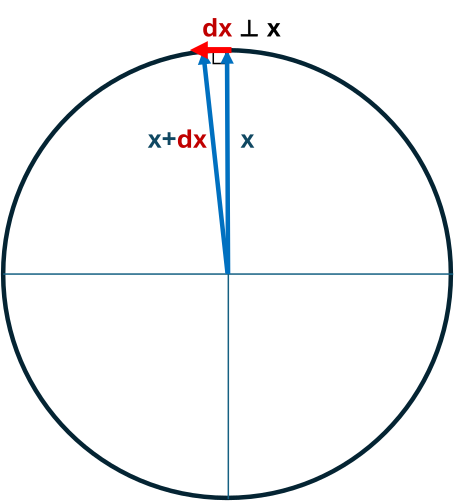
\includegraphics[width=0.3\textwidth]
    {figures/tangent_to_radius.pdf}
    \caption{Differentials on a sphere ($x^T x = 1$): the differential $dx$ is constrained to be perpendicular to $x$.}
    \label{fig:tangentcircle}
\end{figure}

\subsubsection{Special Case: A Circle}

Let us simply consider the unit circle in the plane where $x = (\cos \theta, \sin \theta)$ for some $\theta \in [0,2\pi)$. Then, 
\[
x^T \d x = (\cos \theta, \sin \theta) \cdot (-\sin \theta, \cos \theta) d\theta = 0.
\]
Here, we can think of $x$ as ``extrinsic'' coordinates, in that it is a vector in $\R^2$. On the other hand, $\theta$ is an ``intrinsic'' coordinate, as every point on the circle is specified by one $\theta$.

\subsubsection{On the Sphere}

You may remember that the rank-1 matrix $x x^T$, for any unit vector $x^T x = 1$, is a \textbf{projection matrix} (meaning that it is equal to its square and it is symmetric) which projects vectors onto their components in the direction of $x$.  Correspondingly, $I - x x^T$ is also a projection matrix, but onto the directions \emph{perpendicular} to $x$: geometrically, the matrix removes components in the $x$ direction. In particular, if $x^T \d x= 0$, then $(I - x x^T) \d x = \d x.$ It follows that if $x^T \d x = 0$ and $A$ is a symmetric matrix, we have 
\begin{align*}
    \d \left(\frac{1}{2} x^T A x\right) &= (A x)^T \d x \\
    &= x^T A (\d x) \\
    &= x^T A ( I - x x^T) \d x  \\
    &= ((I - x x^T) A x )^T \d x.
\end{align*}
In other words, $(I - x x^T)A x$ is the gradient of $\frac{1}{2} x^T A x$ \textit{on the sphere.}

So what did we just do? To obtain the gradient on the sphere, we needed (i) a linearization of the function that is correct on tangents, and (ii) a direction that \textit{is} tangent (i.e.~satisfies the linearized constraint). Using this, we obtain the gradient of a general scalar function on the sphere:

\begin{theorem}
    Given $f: \mathbb{S}^n \to \R$, we have 
    \[
    \d f = g(x)^T \d x = (( I - x x^T) g(x))^T \d x.
    \]
\end{theorem}

The proof of this is precisely the same as we did before for $f(x) = \frac{1}{2} x^T A x$.

\subsection{Differentiating on Orthogonal Matrices}

Let $Q$ be an orthogonal matrix. Then, computationally (as is done in the Julia notebook), one can see that $Q^T \d Q$ is an anti-symmetric matrix (sometimes called skew-symmetric). 
\begin{definition}
A matrix $M$ is anti-symmetric if $M = - M^T$. Note that all anti-symmetric matrices thus have zeroes on their diagonals.
\end{definition}

In fact, we can prove that $Q^T \d Q$ is anti-symmetric.
\begin{theorem}
    Given $Q$ is an orthogonal matrix, we have that $Q^T \d Q$ is anti-symmetric.
\end{theorem}

\begin{proof}
    The constraint of being orthogonal implies that $Q^T Q = I$. Differentiating this equation, we obtain 
    \[
    Q^T \d Q + \d Q^T \, Q = 0 \implies Q^T \d Q = - (Q^T \d Q)^T.
    \]
    This is precisely the definition of being anti-symmetric.
\end{proof}

Before we move on, we may ask what the dimension of the ``surface'' of orthogonal matrices is in $\R^{n^2}$.

When $n = 2$, all orthogonal matrices are rotations and reflections, and rotations have the form 
\[
Q = \begin{pmatrix}
    \cos \theta & \sin \theta \\ 
    - \sin \theta & \cos \theta
\end{pmatrix}.
\]
Hence, when $n=2$ we have one parameter.

When $n = 3$, airplane pilots know about ``roll, pitch, and yaw'', which are the three parameters for the orthogonal matrices when $n =3.$ In general, in $\R^{n^2}$, the orthogonal group has dimension $n(n-1)/2$.

There are a few ways to see this.
\begin{itemize}
    \item Firstly, orthogonality $Q^T Q = I$ imposes $n(n+1)/2$ constraints, leaving $n(n-1)/2$ free parameters.
    \item When we do $QR$ decomposition, the $R$ ``eats'' up $n(n+1)/2$ of the parameters, again leaving $n(n-1)/2$ for $Q$.
    \item Lastly, If we think about the symmetric eigenvalue problem where $S = Q \Lambda Q^T$, $S$ has $n(n+1) /2$ parameters and $\Lambda$ has $n$, so $Q$ has $n(n-1)/2$.
\end{itemize}

\subsubsection{Differentiating the Symmetric Eigendecomposition}

Let $S$ be a symmetric matrix, $\Lambda$ be diagonal containing eigenvalues of $S$, and $Q$ be orthogonal with column vectors as eigenvectors of $S$ such that $S = Q \Lambda Q^T$.  [For simplicity, let's assume that the eigenvalues are ``simple'' (multiplicity~1); repeated eigenvalues turn out to greatly complicate the analysis of perturbations because of the ambiguity in their eigenvector basis.] Then, we have 
\[
\d S = \d Q \, \Lambda Q^T + Q \, \d \Lambda \, Q^T + Q \Lambda \d Q^T,
\]
which may be written as 
\[
Q^T \d S \, Q = Q^T \d Q \Lambda - \Lambda Q^T \d Q + \d \Lambda.
\]

As an exercise, one may check that the left and right hand sides of the above are both symmetric. This may be easier if one looks at the diagonal entries on their own, as there $(Q^T \d S \, Q)_{ii} = q_i^T \d S \, q_i$. Since $q_i$ is the $i$th eigenvector, this implies $q_i^T \d S\, q_i = \d \lambda_i.$   (In physics, this is sometimes called the ``Hellman--Feynman'' theorem, or non-degenerate first-order eigenvalue-perturbation theory.)

Sometimes we think of a curve of matrices $S(t)$ depending on a parameter such as time. If we ask for $\frac{\d \lambda_i }{\d t}$, this implies it is thus equal to $q_i^T \frac{ \d S(t)}{\d t} q_i.$ So how can we get the gradient $\nabla \lambda_i$ for one of the eigenvalues? Well, firstly, note that 
\[
\tr (q_i q_i^T)^T \d S) = \d \lambda_i \implies \nabla \lambda_i = q_i q_i^T.
\]

What about the eigenvectors? Those come from off diagonal elements, where for $i \neq j,$
\[
(Q^T \d S \, Q)_{ij} = \left(Q^T \frac{\d Q}{
\d t}\right)_{ij} (\lambda_j - \lambda_i).
\]
Therefore, we can form the elements of $Q^T \frac{\d Q}{ \d t}$, and left multiply by $Q$ to obtain $\frac{\d Q}{\d t}$ (as $Q$ is orthogonal).

It is interesting to get the second derivative of eigenvalues when moving along a line in symmetric matrix space. For simplicity, suppose $\Lambda$ is diagonal and $S(t) = \Lambda + t E.$ Therefore, differentiating
\[
\frac{\d \Lambda}{\d t} = \diag\left(Q^T \frac{\d S(t)}{\d t} Q\right),
\]
we get 
\[
\frac{\d^2 \Lambda}{\d t^2} = \diag \left(Q^T \frac{\d^2 S(t)}{\d t^2} Q\right) + 2 \diag \left(Q^T \frac{\d S(t)}{\d t} \frac{\d Q}{\d t}\right).
\]
Evaluating this at $Q = I$ and recognizing the first term is zero as we are on a line, we have that 
\[
\frac{\d^2 \Lambda}{\d t^2} = 2 \diag \left(E \cdot  \frac{\d Q}{\d t}\right),
\]
or 
\[
\frac{\d^2 \Lambda}{\d t^2} = 2 \sum_{k \neq i} E_{ik}^2/(\lambda_i - \lambda_k).
\]
Using this, we can write out the eigenvalues as a Taylor series: 
\[
\lambda_i (\epsilon) = \lambda_i + \epsilon E_{ii} + \epsilon^2 \sum_{k \neq i} E_{ik}^2/(\lambda_i - \lambda_k) + \dots.
\]
(In physics, this is known as second-order eigenvalue perturbation theory.)